% Options for packages loaded elsewhere
\PassOptionsToPackage{unicode}{hyperref}
\PassOptionsToPackage{hyphens}{url}
\PassOptionsToPackage{dvipsnames,svgnames,x11names}{xcolor}
%
\documentclass[
]{article}

\usepackage{amsmath,amssymb}
\usepackage{iftex}
\ifPDFTeX
  \usepackage[T1]{fontenc}
  \usepackage[utf8]{inputenc}
  \usepackage{textcomp} % provide euro and other symbols
\else % if luatex or xetex
  \usepackage{unicode-math}
  \defaultfontfeatures{Scale=MatchLowercase}
  \defaultfontfeatures[\rmfamily]{Ligatures=TeX,Scale=1}
\fi
\usepackage{lmodern}
\ifPDFTeX\else  
    % xetex/luatex font selection
\fi
% Use upquote if available, for straight quotes in verbatim environments
\IfFileExists{upquote.sty}{\usepackage{upquote}}{}
\IfFileExists{microtype.sty}{% use microtype if available
  \usepackage[]{microtype}
  \UseMicrotypeSet[protrusion]{basicmath} % disable protrusion for tt fonts
}{}
\makeatletter
\@ifundefined{KOMAClassName}{% if non-KOMA class
  \IfFileExists{parskip.sty}{%
    \usepackage{parskip}
  }{% else
    \setlength{\parindent}{0pt}
    \setlength{\parskip}{6pt plus 2pt minus 1pt}}
}{% if KOMA class
  \KOMAoptions{parskip=half}}
\makeatother
\usepackage{xcolor}
\setlength{\emergencystretch}{3em} % prevent overfull lines
\setcounter{secnumdepth}{-\maxdimen} % remove section numbering
% Make \paragraph and \subparagraph free-standing
\ifx\paragraph\undefined\else
  \let\oldparagraph\paragraph
  \renewcommand{\paragraph}[1]{\oldparagraph{#1}\mbox{}}
\fi
\ifx\subparagraph\undefined\else
  \let\oldsubparagraph\subparagraph
  \renewcommand{\subparagraph}[1]{\oldsubparagraph{#1}\mbox{}}
\fi

\usepackage{color}
\usepackage{fancyvrb}
\newcommand{\VerbBar}{|}
\newcommand{\VERB}{\Verb[commandchars=\\\{\}]}
\DefineVerbatimEnvironment{Highlighting}{Verbatim}{commandchars=\\\{\}}
% Add ',fontsize=\small' for more characters per line
\usepackage{framed}
\definecolor{shadecolor}{RGB}{241,243,245}
\newenvironment{Shaded}{\begin{snugshade}}{\end{snugshade}}
\newcommand{\AlertTok}[1]{\textcolor[rgb]{0.68,0.00,0.00}{#1}}
\newcommand{\AnnotationTok}[1]{\textcolor[rgb]{0.37,0.37,0.37}{#1}}
\newcommand{\AttributeTok}[1]{\textcolor[rgb]{0.40,0.45,0.13}{#1}}
\newcommand{\BaseNTok}[1]{\textcolor[rgb]{0.68,0.00,0.00}{#1}}
\newcommand{\BuiltInTok}[1]{\textcolor[rgb]{0.00,0.23,0.31}{#1}}
\newcommand{\CharTok}[1]{\textcolor[rgb]{0.13,0.47,0.30}{#1}}
\newcommand{\CommentTok}[1]{\textcolor[rgb]{0.37,0.37,0.37}{#1}}
\newcommand{\CommentVarTok}[1]{\textcolor[rgb]{0.37,0.37,0.37}{\textit{#1}}}
\newcommand{\ConstantTok}[1]{\textcolor[rgb]{0.56,0.35,0.01}{#1}}
\newcommand{\ControlFlowTok}[1]{\textcolor[rgb]{0.00,0.23,0.31}{#1}}
\newcommand{\DataTypeTok}[1]{\textcolor[rgb]{0.68,0.00,0.00}{#1}}
\newcommand{\DecValTok}[1]{\textcolor[rgb]{0.68,0.00,0.00}{#1}}
\newcommand{\DocumentationTok}[1]{\textcolor[rgb]{0.37,0.37,0.37}{\textit{#1}}}
\newcommand{\ErrorTok}[1]{\textcolor[rgb]{0.68,0.00,0.00}{#1}}
\newcommand{\ExtensionTok}[1]{\textcolor[rgb]{0.00,0.23,0.31}{#1}}
\newcommand{\FloatTok}[1]{\textcolor[rgb]{0.68,0.00,0.00}{#1}}
\newcommand{\FunctionTok}[1]{\textcolor[rgb]{0.28,0.35,0.67}{#1}}
\newcommand{\ImportTok}[1]{\textcolor[rgb]{0.00,0.46,0.62}{#1}}
\newcommand{\InformationTok}[1]{\textcolor[rgb]{0.37,0.37,0.37}{#1}}
\newcommand{\KeywordTok}[1]{\textcolor[rgb]{0.00,0.23,0.31}{#1}}
\newcommand{\NormalTok}[1]{\textcolor[rgb]{0.00,0.23,0.31}{#1}}
\newcommand{\OperatorTok}[1]{\textcolor[rgb]{0.37,0.37,0.37}{#1}}
\newcommand{\OtherTok}[1]{\textcolor[rgb]{0.00,0.23,0.31}{#1}}
\newcommand{\PreprocessorTok}[1]{\textcolor[rgb]{0.68,0.00,0.00}{#1}}
\newcommand{\RegionMarkerTok}[1]{\textcolor[rgb]{0.00,0.23,0.31}{#1}}
\newcommand{\SpecialCharTok}[1]{\textcolor[rgb]{0.37,0.37,0.37}{#1}}
\newcommand{\SpecialStringTok}[1]{\textcolor[rgb]{0.13,0.47,0.30}{#1}}
\newcommand{\StringTok}[1]{\textcolor[rgb]{0.13,0.47,0.30}{#1}}
\newcommand{\VariableTok}[1]{\textcolor[rgb]{0.07,0.07,0.07}{#1}}
\newcommand{\VerbatimStringTok}[1]{\textcolor[rgb]{0.13,0.47,0.30}{#1}}
\newcommand{\WarningTok}[1]{\textcolor[rgb]{0.37,0.37,0.37}{\textit{#1}}}

\providecommand{\tightlist}{%
  \setlength{\itemsep}{0pt}\setlength{\parskip}{0pt}}\usepackage{longtable,booktabs,array}
\usepackage{calc} % for calculating minipage widths
% Correct order of tables after \paragraph or \subparagraph
\usepackage{etoolbox}
\makeatletter
\patchcmd\longtable{\par}{\if@noskipsec\mbox{}\fi\par}{}{}
\makeatother
% Allow footnotes in longtable head/foot
\IfFileExists{footnotehyper.sty}{\usepackage{footnotehyper}}{\usepackage{footnote}}
\makesavenoteenv{longtable}
\usepackage{graphicx}
\makeatletter
\def\maxwidth{\ifdim\Gin@nat@width>\linewidth\linewidth\else\Gin@nat@width\fi}
\def\maxheight{\ifdim\Gin@nat@height>\textheight\textheight\else\Gin@nat@height\fi}
\makeatother
% Scale images if necessary, so that they will not overflow the page
% margins by default, and it is still possible to overwrite the defaults
% using explicit options in \includegraphics[width, height, ...]{}
\setkeys{Gin}{width=\maxwidth,height=\maxheight,keepaspectratio}
% Set default figure placement to htbp
\makeatletter
\def\fps@figure{htbp}
\makeatother
% definitions for citeproc citations
\NewDocumentCommand\citeproctext{}{}
\NewDocumentCommand\citeproc{mm}{%
  \begingroup\def\citeproctext{#2}\cite{#1}\endgroup}
\makeatletter
 % allow citations to break across lines
 \let\@cite@ofmt\@firstofone
 % avoid brackets around text for \cite:
 \def\@biblabel#1{}
 \def\@cite#1#2{{#1\if@tempswa , #2\fi}}
\makeatother
\newlength{\cslhangindent}
\setlength{\cslhangindent}{1.5em}
\newlength{\csllabelwidth}
\setlength{\csllabelwidth}{3em}
\newenvironment{CSLReferences}[2] % #1 hanging-indent, #2 entry-spacing
 {\begin{list}{}{%
  \setlength{\itemindent}{0pt}
  \setlength{\leftmargin}{0pt}
  \setlength{\parsep}{0pt}
  % turn on hanging indent if param 1 is 1
  \ifodd #1
   \setlength{\leftmargin}{\cslhangindent}
   \setlength{\itemindent}{-1\cslhangindent}
  \fi
  % set entry spacing
  \setlength{\itemsep}{#2\baselineskip}}}
 {\end{list}}
\usepackage{calc}
\newcommand{\CSLBlock}[1]{\hfill\break\parbox[t]{\linewidth}{\strut\ignorespaces#1\strut}}
\newcommand{\CSLLeftMargin}[1]{\parbox[t]{\csllabelwidth}{\strut#1\strut}}
\newcommand{\CSLRightInline}[1]{\parbox[t]{\linewidth - \csllabelwidth}{\strut#1\strut}}
\newcommand{\CSLIndent}[1]{\hspace{\cslhangindent}#1}

\usepackage[utf8]{inputenc}
\usepackage[autostyle=true]{csquotes}
\usepackage[colorinlistoftodos, textsize=tiny]{todonotes} % insertar comentarios y notas
% \usepackage[disable]{todonotes} # descomentar si quieres QUITAR notas y comentarios

% \usepackage{acro}
% \ac \Ac acronym first time
% \acs \Acs short form
% \acl \Acl longform

% \acsetup{
% 	make-links = true 
% 	}

% \DeclareAcronym{5-ht}{
%     short = 5-HT,
%     long = Serotonina
% }

% \DeclareAcronym{5-htp}{
%     short = 5-HTP,
%     long = 5-Hidroxitriptófano
% }


%----------------------------------------------------------------------------------------
%	MARGINS
%----------------------------------------------------------------------------------------

% Márgenes para impresión
% \geometry{
% 	headheight=4ex,
% 	includehead,
% 	includefoot
% }

% Márgenes para web
% \geometry{
%     left=2.5cm,
%     right=2.5cm,
%     top=2.5cm,
%     bottom=2.5cm
% }


% \raggedbottom

% \AtBeginDocument{
% \hypersetup{pdftitle=\ttitle} % Set the PDF's title to your title
% \hypersetup{pdfauthor=\authorname} % Set the PDF's author to your name
% \hypersetup{pdfkeywords=\keywordnames} % Set the PDF's keywords to your keywords
% }
\makeatletter
\@ifpackageloaded{caption}{}{\usepackage{caption}}
\AtBeginDocument{%
\ifdefined\contentsname
  \renewcommand*\contentsname{Table of contents}
\else
  \newcommand\contentsname{Table of contents}
\fi
\ifdefined\listfigurename
  \renewcommand*\listfigurename{List of Figures}
\else
  \newcommand\listfigurename{List of Figures}
\fi
\ifdefined\listtablename
  \renewcommand*\listtablename{List of Tables}
\else
  \newcommand\listtablename{List of Tables}
\fi
\ifdefined\figurename
  \renewcommand*\figurename{Figure}
\else
  \newcommand\figurename{Figure}
\fi
\ifdefined\tablename
  \renewcommand*\tablename{Table}
\else
  \newcommand\tablename{Table}
\fi
}
\@ifpackageloaded{float}{}{\usepackage{float}}
\floatstyle{ruled}
\@ifundefined{c@chapter}{\newfloat{codelisting}{h}{lop}}{\newfloat{codelisting}{h}{lop}[chapter]}
\floatname{codelisting}{Listing}
\newcommand*\listoflistings{\listof{codelisting}{List of Listings}}
\makeatother
\makeatletter
\makeatother
\makeatletter
\@ifpackageloaded{caption}{}{\usepackage{caption}}
\@ifpackageloaded{subcaption}{}{\usepackage{subcaption}}
\makeatother
\ifLuaTeX
  \usepackage{selnolig}  % disable illegal ligatures
\fi
\usepackage{bookmark}

\IfFileExists{xurl.sty}{\usepackage{xurl}}{} % add URL line breaks if available
\urlstyle{same} % disable monospaced font for URLs
\hypersetup{
  pdftitle={Unam-quarto Template},
  pdfauthor={string},
  pdfkeywords={template, demo},
  colorlinks=true,
  linkcolor={blue},
  filecolor={Maroon},
  citecolor={Blue},
  urlcolor={Blue},
  pdfcreator={LaTeX via pandoc}}

\title{Unam-quarto Template}

% \programa{Posgrado en Ciencias Biológicas}

% % \facultad{Facultad de Ciencias} % Nombre de la facultad
% 
% +
% \departmento{Biología Experimental} % Nombre del departamento
% 

% % \grado{MAESTRO EN CIENCIAS BIOLÓGICAS}
% 
% % \supervisor{Dr.~Narcissus}
% 
% % \supervisorfac{Thespiae in Boeotia}
% 
% 
% 
% 
% 


% % \author{string}
% 


% 
% % \university{}
% 


% % \group{}
% 

% \setcounter{tocdepth}{3} % The depth to which the document sections are printed to the table of contents

% %   \author{string}{%
%   % 
\begin{document}

% \frontmatter % Use roman page numbering style (i, ii, iii, iv...) for the pre-content pages

\pagestyle{plain} % Default to the plain heading style until the tesis style is called for the body content

%----------------------------------------------------------------------------------------
%	PORTADA
%----------------------------------------------------------------------------------------

% Primera portada
\begin{titlepage}
    \begin{center}
        \vspace*{-1.5cm} % Ajusta este valor conforme sea necesario
        
        % Logo de la UNAM
        
\includegraphics[width=3.5cm]{ figuras/unam.png }\\[0.5cm]
        
        % Nombre de la Universidad
        {\large \textbf{UNIVERSIDAD NACIONAL AUTÓNOMA DE MÉXICO}}\\[0.4cm]
        
        % Programa de posgrado
        {\large \textbf{\MakeUppercase{Posgrado en Ciencias
Biológicas}}}\\[0.3cm]
        
        % Facultad y área
        {\large \MakeUppercase{Facultad de Ciencias}}\\[0.2cm]
        {\large \MakeUppercase{Biología Experimental}}\\[1cm]
        
        % Título de la tesis
        {\Large \textbf{\title}}\\[1cm]
        
        % Texto "Tesis"
        {\LARGE \textbf{T E S I S}}\\[0.5cm]
        
        % Texto de grado
        {\large QUE PARA OPTAR POR EL GRADO DE:}\\[0.3cm]
        {\Large \textbf{MAESTRO EN CIENCIAS BIOLÓGICAS}}\\[1cm]
        
        % Autor
        {\large PRESENTA:}\\[0.3cm]
        {\LARGE \textbf{Santiago García-Rios}}\\[1.0cm]
        
        % Tutor y comité
        {\small \textbf{TUTOR PRINCIPAL DE TESIS:}}\\
        {\small  Dr.~Narcissus }\\
        {\small  Thespiae in Boeotia }\\[0.5cm]
        
        {\small \textbf{COMITÉ TUTOR:}}\\
        {\small  Dr.~Socrates }\\
        {\small  Academy of Athens }\\[0.3cm]
        {\small  Dr.~Plato }\\
        {\small  Academy of Athens }\\[1cm]
        
        % Lugar y fecha
        % \vfill
        %         
    \end{center}
\end{titlepage}


% Primera página de \missingfigure
\newpage
\begin{center}
    \missingfigure[figcolor=white]{\MakeUppercase{\LARGE{Página reservada para Derechos de Autor por parte de la Dirección de Bibliotecas.}}}
\end{center}

% Tercera página de \missingfigure
\newpage
\begin{center}
    \missingfigure{\MakeUppercase{\LARGE{Página reservada para Oficio de Jurado.}}}
\end{center}


\newpage
% \begin{agradecimientos}
    \begin{center}
        
\includegraphics[width=3.5cm]{ figuras/unam.png }\\[0.5cm]
        Este trabajo de Maestría se realizó gracias al Posgrado en Ciencias Biológicas de la Universidad Nacional Autónoma de México (UNAM) y al financiamiento otorgado por el Consejo Nacional de Ciencia y Tecnología (CONACyT) a través de la beca al CVU 1191018 y al proyecto PAPIIT IA205723.

        Deseo expresar mi más sincero agradecimiento a la Universidad Nacional Autónoma de México por haberme recibido nuevamente como parte de su comunidad estudiantil. 
        
        Quiero extender mi agradecimiento a la Facultad de Ciencias de la UNAM por brindar las facilidades y al Laboratorio de Biología Animal Experimental por proporcionar las instalaciones, el equipo y las cámaras. Agradezco al director de esta tesis, el Dr. Alonso, por sus ayudas.
        
        Quiero expresar mi más sincero agradecimiento a todos los miembros del jurado y, en especial, al comité tutoral, el Dr. Jean Pascal Morin y la Dra. María de la Luz Navarro, por dedicar su tiempo a leer esta tesis y proporcionar valiosos comentarios que enriquecieron este trabajo. Su apoyo constante y sus observaciones constructivas fueron fundamentales para lograr un mejor resultado. Gracias por su compromiso y generosidad a lo largo de este proceso.
        
        Por último, gracias a los investigadores y estudiantes que ayudaron a darle forma a este trabajo: gracias a la Dra. Angélica Zepeda y su equipo de trabajo por enseñarme y guiarme con los temas de neurogénesis. Gracias a la Dra. Julieta Rosell García y a los Maestros Diego Ángeles Valdez y Jalil Rasgado Toledo por ser quienes ayudaron con toda la parte de estadística. Gracias los doctores Dan Chitwood y Sarah Percival por incluirme en sus proyectos, donde aprendí muchísimo sobre programación y estadística. Por último, gracias las psicólogas Amanda Sánchez Pérez y Jimena Arroyo Pérez por ayudarme con la parte de trastornos, comportamiento, experimentos y ser quienes discutían y revisaban el proyecto conmigo. Sin ustedes no hubiera sido posible realizar este trabajo.
    \end{center}
% \end{agradecimientos}


\newpage
\begin{center}
    \missingfigure[figcolor=white]{\MakeUppercase{\LARGE{Página en blanco.}}}
\end{center}
\renewcommand*\contentsname{Table of contents}
{
\hypersetup{linkcolor=}
\setcounter{tocdepth}{3}
\tableofcontents
}
\subsection{El Narcisista que Llevas Dentro (Aunque Digas que No):
Cuando el Cerebro se Cree el Protagonista de una
Telenovela}\label{el-narcisista-que-llevas-dentro-aunque-digas-que-no-cuando-el-cerebro-se-cree-el-protagonista-de-una-telenovela}

\subsection{Introduction}\label{sec-intro}

Imagina a esa persona que publica ``Ugh, odio ser tan perfeccionista''
en LinkedIn mientras bebe un latte de oro. Bienvenido al narcisismo
encubierto: el arte de disfrazar la autoimportancia bajo un manto de
falsa modestia. Aquí exploraremos cómo el cerebro de estos individuos
convierte la autocrítica en un humblebrag (autoelogio disfrazado de
queja) y por qué sus neuronas parecen organizar un festival de cine en
su honor.

\emph{TODO} Create a template that demonstrates the appearance,
formatting, layout, and functionality of your format. Learn more about
journal formats at \url{https://quarto.org/docs/journals/}. (Cameron and
Trivedi 2013).

\begin{quote}
In Quarto, we can do these by setting the fig-env command to figure* or
SCfigure*
\end{quote}

\begin{figure}

\centering{


\includegraphics[width=2.67in,height=\textheight]{figuras/unam.png}

}

\caption{\label{fig-side}This legend would be placed at the side of the
figure, rather than below it.}

\end{figure}%

\begin{Shaded}
\begin{Highlighting}[]
\FunctionTok{library}\NormalTok{(tidyverse)}
\end{Highlighting}
\end{Shaded}

\begin{verbatim}
-- Attaching core tidyverse packages ------------------------ tidyverse 2.0.0 --
v dplyr     1.1.3     v readr     2.1.4
v forcats   1.0.0     v stringr   1.5.0
v ggplot2   3.4.4     v tibble    3.2.1
v lubridate 1.9.3     v tidyr     1.3.0
v purrr     1.0.2     
-- Conflicts ------------------------------------------ tidyverse_conflicts() --
x dplyr::filter() masks stats::filter()
x dplyr::lag()    masks stats::lag()
i Use the conflicted package (<http://conflicted.r-lib.org/>) to force all conflicts to become errors
\end{verbatim}

\begin{Shaded}
\begin{Highlighting}[]
\NormalTok{df }\OtherTok{\textless{}{-}} \FunctionTok{tibble}\NormalTok{(}\AttributeTok{x =} \DecValTok{1}\SpecialCharTok{:}\DecValTok{10}\NormalTok{, }\AttributeTok{y =} \FunctionTok{rnorm}\NormalTok{(}\DecValTok{10}\NormalTok{))}

\FunctionTok{ggplot}\NormalTok{(df, }\FunctionTok{aes}\NormalTok{(x, y)) }\SpecialCharTok{+}
  \FunctionTok{geom\_point}\NormalTok{()}
\end{Highlighting}
\end{Shaded}

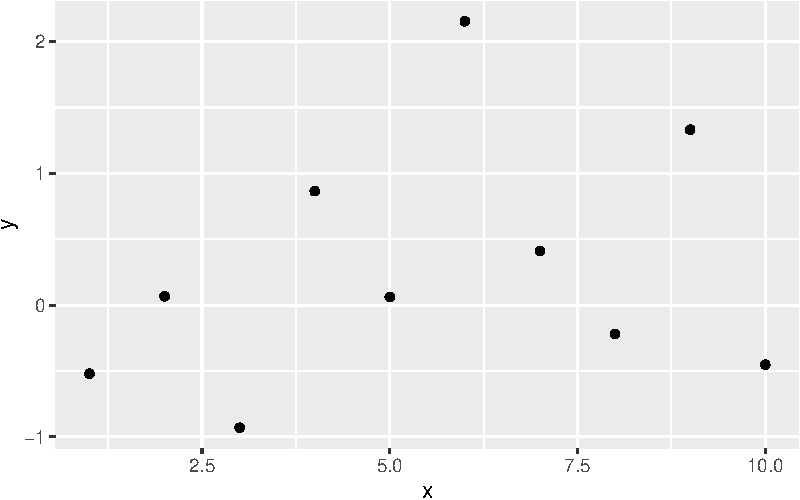
\includegraphics{template_files/figure-pdf/unnamed-chunk-2-1.pdf}

\subsection{Introducción}\label{introducciuxf3n}

\begin{itemize}
\tightlist
\item[$\square$]
  Comenzar con una oración de tópico
  (\href{https://en.wikipedia.org/wiki/Inverted_pyramid_(journalism)}{pirámide
  invertida})
\item[$\square$]
  Revisión concisa de literatura pertinente
\end{itemize}

\href{https://writingcenter.gmu.edu/writing-resources/imrad/imrad-reports-introductions}{Ver
más}

\subsubsection{Tables}\label{tables}

\begin{Shaded}
\begin{Highlighting}[]
\InformationTok{\textasciigrave{}\textasciigrave{}\textasciigrave{}\{r\}}
\InformationTok{\#| label: tbl{-}cars}
\InformationTok{\#| tbl{-}cap: This is my caption.}
\InformationTok{knitr::kable(head(mtcars))}
\InformationTok{\textasciigrave{}\textasciigrave{}\textasciigrave{}}
\end{Highlighting}
\end{Shaded}

The \texttt{\#\textbar{}} is what sets up our cross-references and you
can then reference the table as \texttt{@tbl-cars}. Note in order for
table numbering to work in Quarto, you \textbf{must} label your tables
with the \texttt{tbl-} prefix.

\begin{Shaded}
\begin{Highlighting}[]
\NormalTok{knitr}\SpecialCharTok{::}\FunctionTok{kable}\NormalTok{(}\FunctionTok{head}\NormalTok{(mtcars))}
\end{Highlighting}
\end{Shaded}

\begin{longtable}[]{@{}
  >{\raggedright\arraybackslash}p{(\columnwidth - 22\tabcolsep) * \real{0.2609}}
  >{\raggedleft\arraybackslash}p{(\columnwidth - 22\tabcolsep) * \real{0.0725}}
  >{\raggedleft\arraybackslash}p{(\columnwidth - 22\tabcolsep) * \real{0.0580}}
  >{\raggedleft\arraybackslash}p{(\columnwidth - 22\tabcolsep) * \real{0.0725}}
  >{\raggedleft\arraybackslash}p{(\columnwidth - 22\tabcolsep) * \real{0.0580}}
  >{\raggedleft\arraybackslash}p{(\columnwidth - 22\tabcolsep) * \real{0.0725}}
  >{\raggedleft\arraybackslash}p{(\columnwidth - 22\tabcolsep) * \real{0.0870}}
  >{\raggedleft\arraybackslash}p{(\columnwidth - 22\tabcolsep) * \real{0.0870}}
  >{\raggedleft\arraybackslash}p{(\columnwidth - 22\tabcolsep) * \real{0.0435}}
  >{\raggedleft\arraybackslash}p{(\columnwidth - 22\tabcolsep) * \real{0.0435}}
  >{\raggedleft\arraybackslash}p{(\columnwidth - 22\tabcolsep) * \real{0.0725}}
  >{\raggedleft\arraybackslash}p{(\columnwidth - 22\tabcolsep) * \real{0.0725}}@{}}

\caption{\label{tbl-cars}This is my caption.}

\tabularnewline

\toprule\noalign{}
\begin{minipage}[b]{\linewidth}\raggedright
\end{minipage} & \begin{minipage}[b]{\linewidth}\raggedleft
mpg
\end{minipage} & \begin{minipage}[b]{\linewidth}\raggedleft
cyl
\end{minipage} & \begin{minipage}[b]{\linewidth}\raggedleft
disp
\end{minipage} & \begin{minipage}[b]{\linewidth}\raggedleft
hp
\end{minipage} & \begin{minipage}[b]{\linewidth}\raggedleft
drat
\end{minipage} & \begin{minipage}[b]{\linewidth}\raggedleft
wt
\end{minipage} & \begin{minipage}[b]{\linewidth}\raggedleft
qsec
\end{minipage} & \begin{minipage}[b]{\linewidth}\raggedleft
vs
\end{minipage} & \begin{minipage}[b]{\linewidth}\raggedleft
am
\end{minipage} & \begin{minipage}[b]{\linewidth}\raggedleft
gear
\end{minipage} & \begin{minipage}[b]{\linewidth}\raggedleft
carb
\end{minipage} \\
\midrule\noalign{}
\endhead
\bottomrule\noalign{}
\endlastfoot
Mazda RX4 & 21.0 & 6 & 160 & 110 & 3.90 & 2.620 & 16.46 & 0 & 1 & 4 &
4 \\
Mazda RX4 Wag & 21.0 & 6 & 160 & 110 & 3.90 & 2.875 & 17.02 & 0 & 1 & 4
& 4 \\
Datsun 710 & 22.8 & 4 & 108 & 93 & 3.85 & 2.320 & 18.61 & 1 & 1 & 4 &
1 \\
Hornet 4 Drive & 21.4 & 6 & 258 & 110 & 3.08 & 3.215 & 19.44 & 1 & 0 & 3
& 1 \\
Hornet Sportabout & 18.7 & 8 & 360 & 175 & 3.15 & 3.440 & 17.02 & 0 & 0
& 3 & 2 \\
Valiant & 18.1 & 6 & 225 & 105 & 2.76 & 3.460 & 20.22 & 1 & 0 & 3 & 1 \\

\end{longtable}

This is Table~\ref{tbl-cars}.

See the Quarto manual for full examples and instructions.

\subsubsection{Figures}\label{figures}

Again we write in Quarto (markdown) not \LaTeX{} for our figures. You
can write in \LaTeX{} if you really want but it would only be
interpreted for the PDF output.

\begin{Shaded}
\begin{Highlighting}[]
\InformationTok{\textasciigrave{}\textasciigrave{}\textasciigrave{}\{r\}}
\InformationTok{\#| label: fig{-}cars}
\InformationTok{\#| fig{-}cap: This is my caption.}
\InformationTok{plot(mtcars[,1:4])}
\InformationTok{\textasciigrave{}\textasciigrave{}\textasciigrave{}}
\end{Highlighting}
\end{Shaded}

The \texttt{\#\textbar{}} is what sets up our cross-references and you
can then reference the table as \texttt{@fig-cars}.

\begin{Shaded}
\begin{Highlighting}[]
\FunctionTok{plot}\NormalTok{(mtcars[,}\DecValTok{1}\SpecialCharTok{:}\DecValTok{4}\NormalTok{])}
\end{Highlighting}
\end{Shaded}

\begin{figure}[H]

\centering{

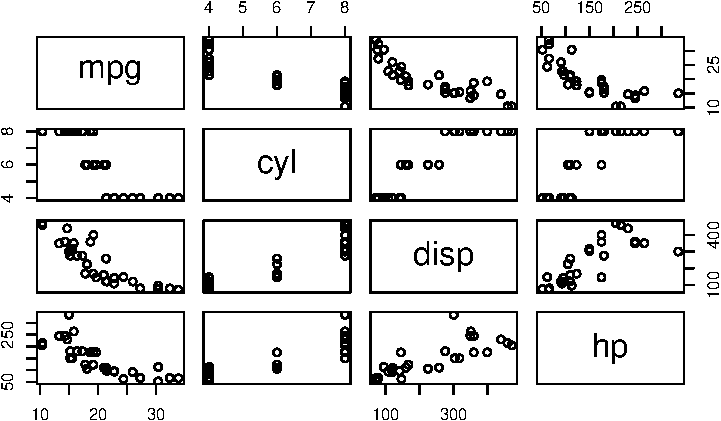
\includegraphics{template_files/figure-pdf/fig-cars-1.pdf}

}

\caption{\label{fig-cars}This is my caption.}

\end{figure}%

This is Figure~\ref{fig-cars}.

See the Quarto manual for full examples and instructions.

\subsection{Planteamiento del
problema}\label{planteamiento-del-problema}

\begin{quote}
¿Cómo detectar a un narcisista encubierto antes de que te invite a su
monólogo sobre lo ``difícil que es ser tan inteligente y sensible''?
\end{quote}

La neurociencia sugiere que sus cerebros podrían tener áreas
hiperactivas en la corteza prefrontal (responsable de la autoevaluación)
y una amígdala que grita ``¡Mírame!'' cada vez que alguien recibe más
likes. ¿Es esto evolución o un bug cerebral?

\subsection{Justificación}\label{justificaciuxf3n}

Estudiar esto es crucial para:

\begin{itemize}
\item
  Evitar que la palabra ``humildad'' sea secuestrada por narcisistas.
\item
  Diseñar apps que detecten mensajes pasivo-agresivos en redes sociales
  (``NeuroFilter: ¿Seguro que quieres publicar eso?'').
\item
  Salvar a la humanidad de conversaciones que empiezan con ``Soy
  demasiado empático, es mi maldición''
\end{itemize}

\subsection{Antecedentes}\label{antecedentes}

\begin{itemize}
\tightlist
\item[$\square$]
  Incluir suficiente literatura para entender la razón y contexto del
  estudio.
\item[$\square$]
  Explicar el enfoque experimental.
\item[$\square$]
  Explicar cómo los animales y modelos se usaron para explorar los
  objetivos científicos.
\item[$\square$]
  Si es relevante, explicar el impacto en la salud humana.
\item[$\square$]
  Comienza por explicar por qué es importante la investigación
\item[$\square$]
  Seguir por explicar el estado actual de la investigación
\item[$\square$]
  Seguir de hoyos o oproblemas en el campo.
\item[$\square$]
  Finalmente explicar cómo el estudio busca una solución a este
  problema.
\end{itemize}

(ChatGPT-10 2024; 2.0 2023; González and Likeador 2019; Hashtag 2020;
TerapiaExpress 2021; Postureo and HumildeFalsa 2022; EgoMeter and
BrainDrama 2023)

\subsection{Objetivos e hipótesis}\label{objetivos-e-hipuxf3tesis}

\begin{itemize}
\item[$\square$]
  pregunta de investigación
\item[$\square$]
  objetivos de la investigación
\item[$\square$]
  hipótesis a probar
\item
  Usar fMRI para encontrar la ``zona del humblebrag'' en el cerebro.
\item
  Medir la actividad de la dopamina cuando alguien les dice ``Wow, eres
  tan auténtico''.
\item
  Crear un test basado en cuántas veces revisan su perfil de Tinder en
  una hora.
\end{itemize}

\begin{quote}
Proponemos que el narcisista encubierto tiene un circuito neuronal que
convierte la autocrítica en combustible para su ego, como un Tamagotchi
que solo come cumplidos indirectos. Su cerebro procesa el ``No soy nada
especial'' como ``Soy el mesías de la modestia''.
\end{quote}

\subsection{Metodolodía}\label{metodoloduxeda}

\emph{Metodología}: Este término es más amplio y no solo describe los
procedimientos específicos utilizados en el experimento, sino también
las bases teóricas que justifican esos métodos. Incluye una discusión
sobre por qué ciertos métodos son apropiados para la investigación en
cuestión. Si tu sección describe tanto el ``cómo'' (los pasos y
procedimientos) como el ``por qué'' (la justificación de la elección de
esos métodos).

\emph{Diseño Experimental}: Este término se refiere específicamente al
plan estructural de la investigación, cómo se organizan los
experimentos, qué variables se controlan, cómo se asignan los sujetos a
diferentes grupos, etc. Es más específico que ``Método'' y se centra en
la planificación del experimento en sí.

\emph{Método}: Es un término más específico y directo. Se enfoca en los
pasos concretos y técnicas empleadas en la investigación, sin
necesariamente entrar en detalles sobre la justificación teórica de esos
métodos.

\begin{itemize}
\tightlist
\item[$\square$]
  Escribir en pasado, con voz pasiva (\emph{Daniel cocinó una tortilla},
  \emph{Una tortilla fue cocinada por Danie}, \emph{Daniel la cocinó},
  \emph{América fue colonizada en 1492}, \emph{Se reparan automóviles
  /Se espera la renuncia del mandatario}), en contraste de voz activa
  (\emph{El presidente pronunció un largo discurso}, \emph{Varios
  millones visitan Barcelona cada año})
\end{itemize}

\begin{longtable}[]{@{}
  >{\raggedright\arraybackslash}p{(\columnwidth - 2\tabcolsep) * \real{0.4516}}
  >{\raggedright\arraybackslash}p{(\columnwidth - 2\tabcolsep) * \real{0.5484}}@{}}
\toprule\noalign{}
\begin{minipage}[b]{\linewidth}\raggedright
\textbf{Voz Activa}
\end{minipage} & \begin{minipage}[b]{\linewidth}\raggedright
\textbf{Voz Pasiva}
\end{minipage} \\
\midrule\noalign{}
\endhead
\bottomrule\noalign{}
\endlastfoot
El presidente pronunció un largo discurso & Un largo discurso fue
pronunciado por el presidente \\
Varios millones visitan Barcelona cada año & Barcelona es visitada cada
año por varios millones \\
Mi madre horneó una tarta de chocolate & Una tarta de chocolate fue
horneada por mi madre \\
Unos ladrones atracaron el banco & El banco fue atracado por unos
ladrone \\
\end{longtable}

\begin{longtable}[]{@{}ll@{}}
\toprule\noalign{}
\textbf{Verbo Activo} & \textbf{Verbo Pasivo} \\
\midrule\noalign{}
\endhead
\bottomrule\noalign{}
\endlastfoot
Escribe & Es escrito \\
Escribió & Fue escrito \\
Escribirá & Será escrito \\
Escriba & Sea escrito \\
Han escrito & Han sido escritos \\
\end{longtable}

Animales - {[} {]} cuidado y monitoreo - {[} {]} Aprovación de comité de
ética - {[} {]} Intervenciones y pasos utilizados para reducir dolor,
sufrimiento y distrés. - {[} {]} Cómo se obtuvo el tamaño de la muestra
a priori.

\subsection{Resultados y discusión}\label{resultados-y-discusiuxf3n}

\begin{verbatim}
MRI Funcional: Su corteza prefrontal se ilumina al escribir "Soy un desastre" (traducción neuronal: "Soy un desastre... ¡PERO MÍRENME ARREGLARLO!").

Dopamina: Sube un 300% al recibir comentarios como "Eres tan real, odio a los falsos".

Correlación: A mayor uso de hashtags como #VidaSencilla, mayor actividad en la ínsula (área de la autopercepción dramática).
\end{verbatim}

Nota: Los sujetos negaron todos los resultados, diciendo ``Yo solo estoy
aquí para ayudar a la ciencia'' (clásico).

\subsection{Conclusión}\label{conclusiuxf3n}

Confirmamos que el narcisismo encubierto es como el ajo en las recetas:
todos creen que no lo usan, pero se huele a kilómetros. La neurociencia
sugiere que sus cerebros son máquinas de autoengaño sofisticadas, pero
con suficiente humor y memes, quizá podamos salvarlos (o al menos
reírnos en el proceso). Propuesta final: un bot de Twitter que responda
``Ok, Sigmund Freud'' a sus hilos existenciales.

\phantomsection\label{refs}
\begin{CSLReferences}{1}{0}
\bibitem[\citeproctext]{ref-NeurosisEnPijama2023}
2.0, Freud. 2023. \emph{Neurosis En Pijama: La Neurociencia Del Que Sube
Historias Motivacionales a Las 3 AM}. Silicon Valley: NeuroVanity Press.

\bibitem[\citeproctext]{ref-CameronTrivedi2013}
Cameron, A. Colin, and Pravin K. Trivedi. 2013. \emph{Regression
Analysis of Count Data}. 2nd ed. Cambridge: Cambridge University Press.

\bibitem[\citeproctext]{ref-IAyNarcisismo2024}
ChatGPT-10. 2024. {``¿Puede La {IA} Diagnosticar a Tu Ex? Un Análisis de
Mensajes Pasivo-Agresivos En Tinder.''} Reporte Técnico NTD-007.
Instituto de Tecnologías Dramáticas.

\bibitem[\citeproctext]{ref-FreudRecargado2023}
EgoMeter, Vanessa, and Ludwig BrainDrama. 2023. {``Why Do i Love Me? A
Neural Survey of Self-Admiration.''} \emph{Journal of Questionable
Personality Traits} 42 (6): 1337--50.
\url{https://doi.org/10.1234/jqpt.2023.007}.

\bibitem[\citeproctext]{ref-DopaminaYSelfies2019}
González, Dopamina, and Sergio Likeador. 2019. {``La Curva de La
Dopamina En Publicaciones de Café Artesanal: Un Estudio Con Narcisistas
Encubiertos.''} \emph{Annual Review of Pretentious Behavior} 7: 42--666.
\url{https://doi.org/10.6666/ar.pb.2019.007}.

\bibitem[\citeproctext]{ref-NeuroFilter2020}
Hashtag, Alan. 2020. {``NeuroFilter: Cómo Detectar Un {{`Humblebrag'}}
En 280 Caracteres o Menos.''} In \emph{Memes y Neuronas: La Ciencia
Detrás de Tu Timeline Tóxico}, edited by Twitter Académico, 69--420.
TikTok Academic Publications.

\bibitem[\citeproctext]{ref-SelfieCerebral2022}
Postureo, Carlos, and María HumildeFalsa. 2022. \emph{Humblebrags \&
Brain Scans: {fMRI} No Miente, Tu Perfil de Instagram Sí}. 1st ed.
Colección Para Narcisistas En Recuperación. Berlin: Springer.

\bibitem[\citeproctext]{ref-DejaDeLeer2021}
TerapiaExpress, Ana. 2021. \emph{Deja de Leer Esto y Ve a Terapia: Guía
de Supervivencia Para El Autoengañado Crónico}. Buenos Aires: Ediciones
Ironía Sana.

\end{CSLReferences}



\end{document}
